% !Mode:: "TeX:UTF-8"


\chapter{需求分析}

\section{整体需求分析}
App的主要功能是检测算式,同时可以统计、分析检测过的算式,给学生推荐常出错的习题,帮助学生学习数学。App的用户有老师、学生和管理员三种角色,老师和学生需要注册、登陆功能,管理员有查看、添加和删除用户的需求。
\begin{figure}[h!]
	\centering
	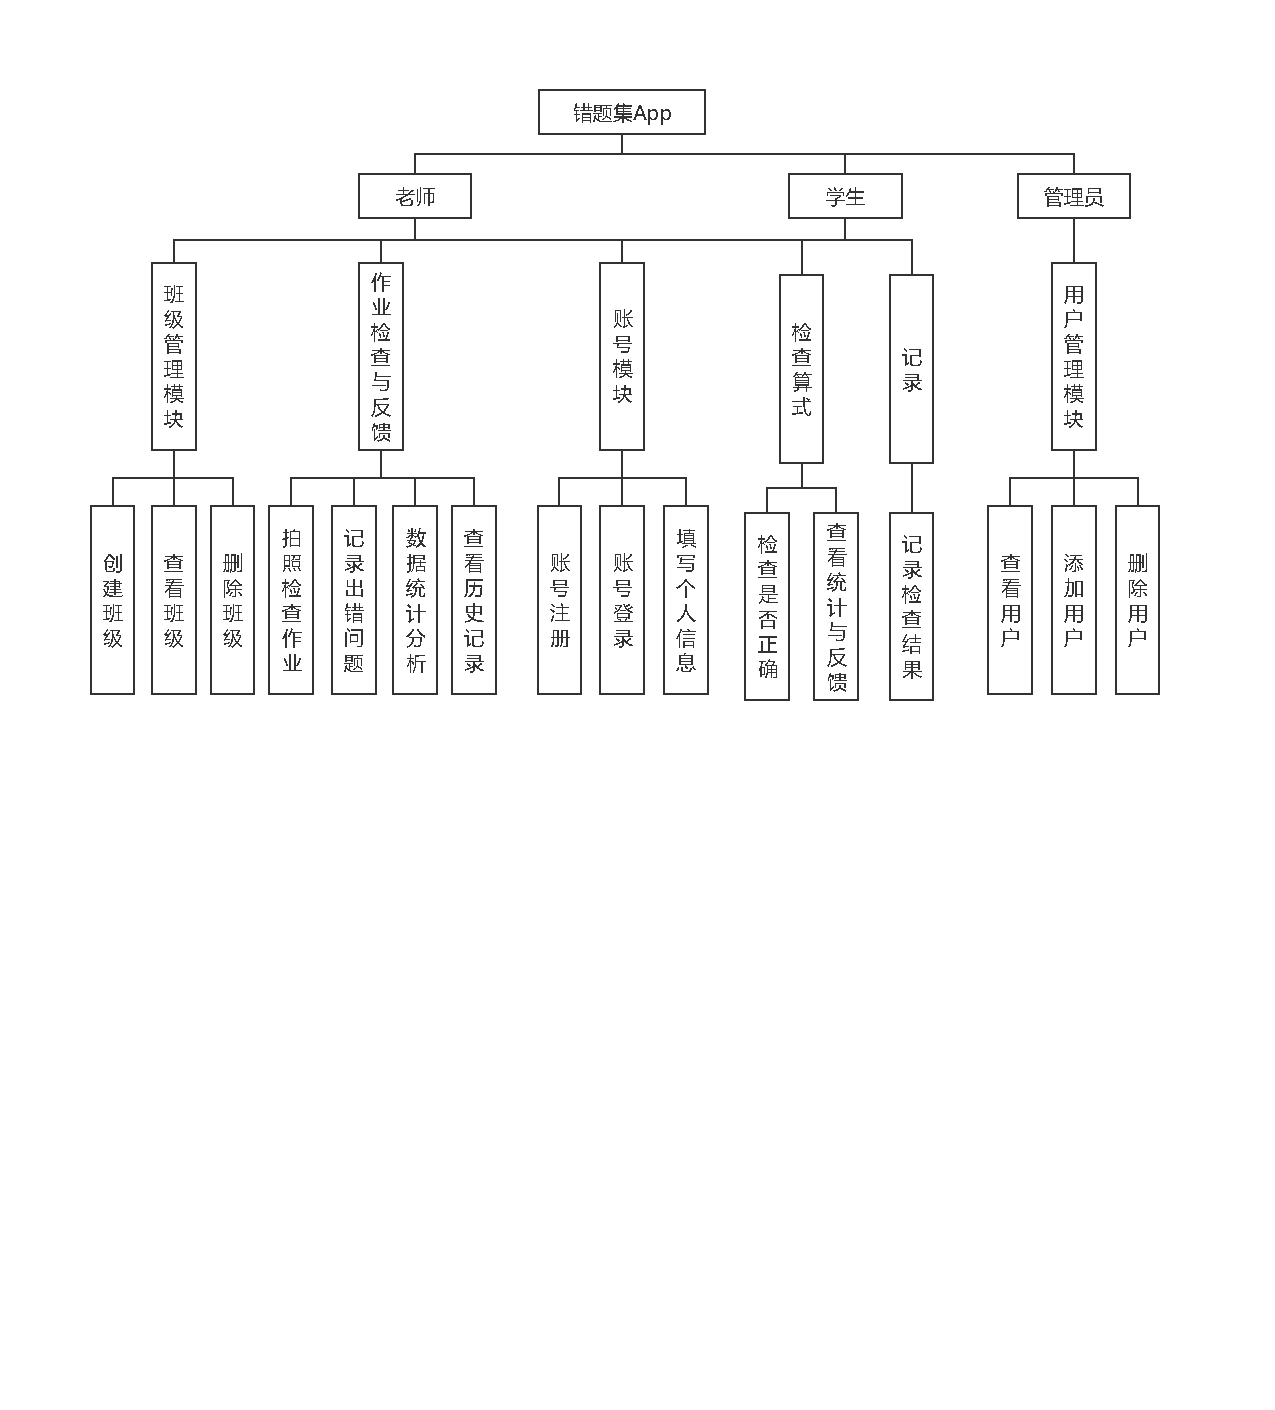
\includegraphics[width=350bp]{picture/overallDemand.pdf}
	\caption{总体需求}
	\label{fig:}
\end{figure}

\section{账号模块需求分析}
用户注册:用户需要提交用户名、密码和email地址,同时选择自己是学生还是老师,注册登陆完成后,用户可以选择进一步完善个人信息,包括姓名、性别、年龄和班级。
\par
用户登陆:用户提交用户名和密码,系统判断是否允许用户登陆,不同角色的用户登陆后,能使用对应的功能。

\section{算式识别模块需求分析}
用户可以选择从本地选择图片或是使用相机拍照,选择图片后上传到服务器,服务器上的识别程序需要判断出每个等式的正误,并在图片上做出相应的标记,识别结束后把结果存储在数据库,同时把结果图片返回客户端,客户端需要把收到的响应呈现在视图层。

\section{错题集模块需求分析}
用户可以看到自己上传的图片处理结果的历史记录和出错题目的统计分析结果。系统会根据用户的历史做题结果提供相似题目的推荐。

\section{本章小结}

